\chapter{Signal Simulation} \label{sec: mgsim}

The MadGraph signal simulation was performed assuming that the mass of the heavy neutrino was 1.5 TeV. Also, taking into the account that the analysis was going to be performed using Vector Boson Fusion, the paramater of minimum pseudorapidity separation ($\Delta \eta$) between two jets was set to 3.5.

The commands used to generate the desired signal were the ones shown in Figure \ref{fig: mgCommands}.

\begin{figure}[H]
\centering
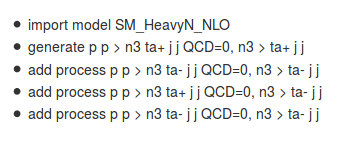
\includegraphics[scale = 1]{Figures/mg_commands}
\caption{MadGraph commands used to generate signal}
\label{fig: mgCommands}
\end{figure}

The first command imports the theoretical model that includes the interactions related with the heavy neutrino formation and decay. The next command specifies the processes that are going to be simulated. pp $>$ n3 ta+ jj stands por the proton-proton collision that decays into a heavy neutrino, a $\tau$ with positive charge, and two jets. The flag QCD=0 is used to exclude all strong interactions that can be involved in the process. Finally, n3 $>$ ta+ jj is used to force the decay of the heavy neutrino into a $\tau$ charge positively and two jets. The subsequent commands are used to take into account all the possible combinations of the electrical charge that the $\tau$ may have.

\begin{figure}[H]
\centering
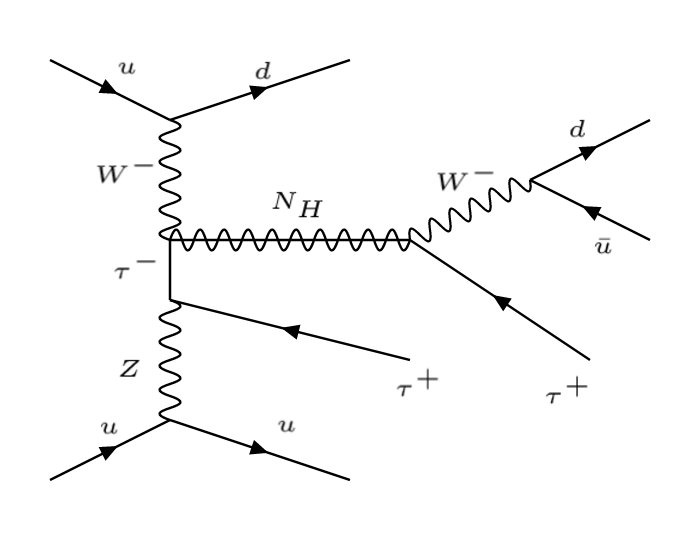
\includegraphics[scale = 0.45]{Figures/Feynman_hnZ}
\caption{Feynman diagram of simulated process involving Z boson}
\label{fig: hnZ}
\end{figure}

Figures \ref{fig: hnZ} and \ref{fig: hnGamma} show two of the main possible diagrams generated by MadGraph for the processes simulated. This two diagrams present a complete picture involving the processes shown in the diagrams of Figures \ref{fig: VBF} and \ref{fig: W}. Figure \ref{fig: VBF} shows the diagram of the vector boson fusion process, ocurring in Figures \ref{fig: hnZ} and \ref{fig: hnGamma} in the fusion of the W boson with the Z boson and the photon ($\gamma$) respectively. In these last two diagrams, the decay of the of the W boson coincides with the one shown in Figure \ref{fig: W} for the decay of the W boson resulting in a heavy neutrino and a lepton, which in this case is a $\tau$.

\begin{figure}[H]
\centering
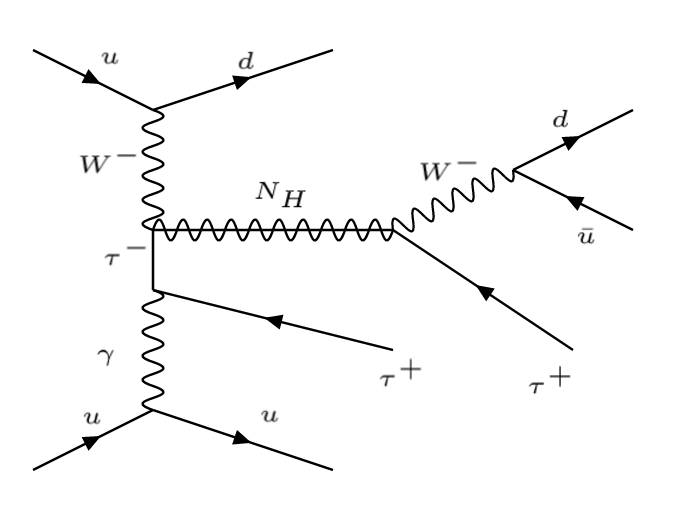
\includegraphics[scale = 0.45]{Figures/Feynman_hnGamma}
\caption{Feynman diagram of simulated process involving photon}
\label{fig: hnGamma}
\end{figure}

The simulation was performed in 10 different simulation batches each one containing 10,000 events. Every batch was generated with a different random seed to guarantee the independence of the events between each one of the generated batches. This independance was necessary because the 10,000 event files were merged to form a single file with 100,000 events. As explained earlier, after the events were simulated in MadGraph they were passed to Pythia and then to Delphes so the signal resembled one that could be found at CMS.  

